\documentclass[12pt, a4paper]{article}
\usepackage[english, serbianc]{babel}
\usepackage{authblk}

\usepackage{amsmath}
\usepackage{amssymb}
\usepackage{graphicx}
\usepackage{amsfonts}

\usepackage{subfig}
\usepackage{float}
\usepackage{booktabs}

\usepackage{siunitx}
\usepackage[%
colorlinks=true,
pdfborder={0 0 0},
linkcolor=red
]{hyperref}

\begin{document}
\date{}
\title{HR аналитика}
\author{Коста Грујчић}
\affil{12/2017}
\maketitle

\begin{abstract}
	Циљ пројекта је истренирати логистичку регресију над подацима о предвиђању одласка запосленог из предузећа на основу великог броја параметара за сваког од њих.
\end{abstract}

\section{Увод}
	Како је у питањеу проблем бинарне класификације, природно је користити метрику прецизности за модел, док се успешност над појединачним класама мери односом одзива и прецизности.
	
	Приметимо да нам је од веће важности предвидети да ће неки запослени напустити предузеће него да он неће. Уколико за запосленог тврдимо да ће он напустити предузеће, његов надређени или неко из HR тима може обавити додатни разговор са њим и тиме утврдити евентуални проблем. С друге стране, уколико за некога тврдимо да ће остати, он одлуку о одласку доноси изненада. С тим у вези, грешке прве и друге врсте нису еквивалентне. Зато је пожељно максимизирати одзив предвиђања одласка запосленог. Како нам је ипак важно да и прецизност буде што је могуће већа, коначан циљ је максимизирати $F_1$ меру те класе.
	
	Надаље ћемо одлазак запосленог звати позитивном класом, јер нам је циљ предвидети је, док ћемо останак запосленог звати негативном класом.

\section{Подаци}
	Подаци који су доступни су подељени у три документа, али како је сваки запослени представљен јединственим идентификатором лако их можемо спојити у један скуп података. Тако добијени скуп података третирамо као табелу чије су колоне називи атрибута, док редове тумачимо као вишедимензионе векторе. Увидом у податке можемо закључити следеће:
	
	\begin{itemize}
		\item Колоне \textsc{Over18}, \textsc{StandardHours} и \textsc{EmployeeCount} можемо уклонити јер су једнаке за све редове у табели.
		\item Присутни су недостајући подаци у појединим колонама.
		\item Постоје нумерички и категорички атрибути.
		\item Негативна и позитивна класа нису равномерно заступљене.
	\end{itemize}
	
	Из матрице корелације (слика \ref{fig:corr}) можемо видети да велики број атрибута нису у корелацији, док и када она евидентно постоји није значајно велика. То додатно отежава одабир релеватних атрибута јер међу њима постоји нелинеарна зависност.
	
	\begin{figure}[H]
		\centering
		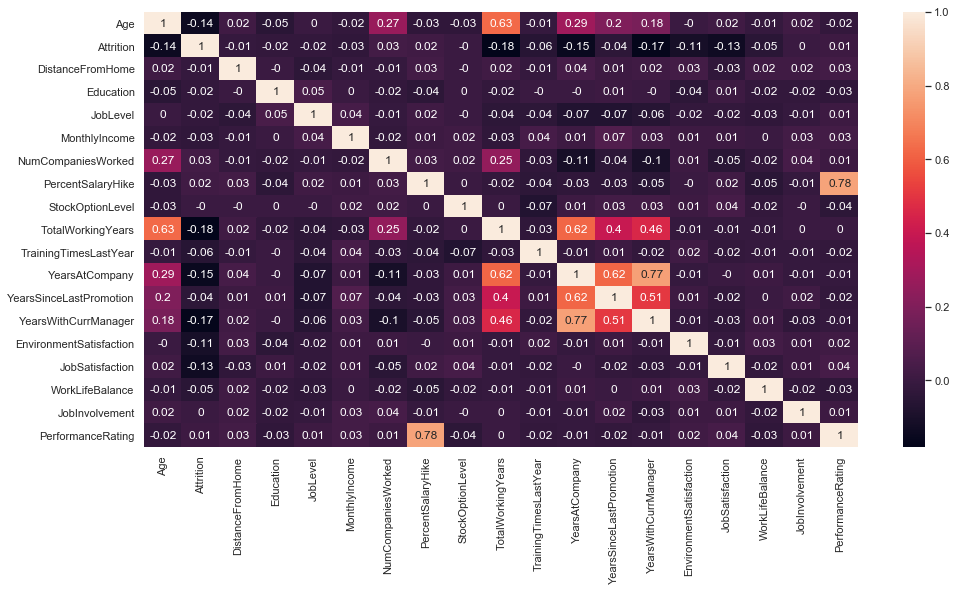
\includegraphics[height=8cm]{graphics/full_correlation.png}
		\caption{матрица корелације нумеричких атрибута}
		\label{fig:corr}
	\end{figure}

\section{Приступ}
	Како је у питању класификациони проблем са две класе, применићемо логистичку регресију. Подаци који су нам на располагању садрже велики број атрибута од којих су неки очекивано ирелевантни. Будући да логистичка регресија не може бити директно примењена на категоричке атрибуте, потребно је извршити њихову трансформацију. Зато ћемо описати одабир својстава и начин трансформисања категоричих атрибута.
	
	Оба поменута проблема се могу решавати независно, али и заједно, те ћемо описати оба поступка и упоредити их. Надање ћемо их редом звати \textit{експлицитни} и \textit{имплицитни} приступ.
	
	\subsection{Увођење помоћних атрибута и експлицитно одстрањивање ирелевантних атрибута} \label{app:1}
	У овом приступу је категоричке атрибуте неопходно пресликати у нумеричке. У ту сврху се такви атрибути пресликавају у ретке векторе који на само једном месту имају јединицу, док су свуда остало нуле. Димензија тог вектора је једнака броју вредности које одговарајући категорички атрибут може имати.

	Конкретно, ако категорички атрбиту има свега две могуће вредности, тада се једна од њих представља вектором $(1, 0)$, а друга $(0, 1)$.

	Овакав приступ не уводи никакав поредак међу векторима јер они чине ортонормирану базу. Међутим, имплицитно је индукована линеарна зависност атрибута, јер важи $\sum_{i} v_i = \textbf{1}$. Због тога се један од вектора мења нула вектором.

	Применом описаног поступка, добијамо $40$ нумеричких атрибута. Њихов број је очигледно превелик и да би се убрзао процес обучавања регресионог модела неке је потребно одстранити. Зато се на основу тренинг скупа, обучава неколико модела који могу проценити релевантност атрибута (попут насумичне шуме одлучивања или метода потпорних вектора). Уколико неки од тих модела одређени атрибут прогласи релевантним, додељује му се један глас. Бирају се сви атрибути са бар $3$ гласа. На тај начин смо број атрибута више него преполовили. Напомињемо да су недостајуће вредности замењене медијаном. Изгласане атрибуте можемо видети у табели...

	Потом се врши обучавање логистичке регресије. Како је потребно контролисати прилагођеност подацима, неопходно је одредити регуларизациони параметар регресионог модела. Како поменути параметар може узети вредност из непребројивог скупа, потребно је вршити узорковање или дискретизацију простора претраге. Опредељујемо се за први приступ и користимо \texttt{BayesSearchCV}. Претпоставља се $\log$-равномерна расподела параметра (у пакету \texttt{sklearn} се зове $C$). То значи да ће се параметар $C$ узорковати из поменуте расподеле и чувати онај који је најбољи у односу на задату метрику. Изводи се $300$ симулација над искључиво тренинг скупом над којим се врши унакрсна валидација ради мерења ваљаности тако изабраног параметра. Бира се параметар за који модел логистичке регресије има највећу површину испод $ROC$ криве. Водимо рачуна да се врши стратификована унакрсна валидација јер су класе неравномерно заступљене. Унакрсну валидацију лако изводимо употребом \texttt{StratifiedKFold} за $k=5$.

	Коначно, тако оптимизован \texttt{LogisticRegression} модел се тренира над тренинг скупом кроз $100$ итерација или до конвергенције. Како постоји изражена неуравнотеженост класа, потребно је форсирати њихово балансирање у регресионом моделу, што на срећу, постоји као могућност у поменутом пакету
	
	\subsection{Имплицитно одстрањивање атрибута без увођења додатних атрибута} \label{app:2}
	
	У претходно описаном поступку, релевантност атрибута је диктирана као хиперпараметар. Као алтернативан приступ, применићемо метод \textit{weight of evidence} који не захтева елиминацију недостајућих вредности, експлицитно мењање категоричких атрибута нумеричким као ни експлицитно бирање релевантних атрибута.
	
	Основна идеја је подела атрибута у дискретне скупове којима се придружује вредност на основу односа заступљености циљне променљиве у њима. Такву вредност зовемо $WOE$ вредност. Затим се она додатно користи за пондерисање релативне заступљености позитивне класе чиме се добија \textit{нформациона вредност} (енг. $IV$) на основу које се може проценити релевантност атрибута.
	
	Дајемо формално извођење поменутог метода. Нека је атрибут $X_j$ подељен на строге подскупове $B_1, ..., B_n$ и нека је $Y$ случајна величина циља. Вредност $$\log\frac{P(X_j \in B_i \mid Y=1)}{P(X_j \in B_i \mid Y=0)}$$ означавамо са $WOE_{i,j}$. Можемо је оценити директно из узорка. Потом, информациону вредност атрибута $X_j$ дефнишемо као $$IV_j = \sum_{i=1}^{n}(P(X_j \in B_i \mid Y=1) - P(X_j \in B_i \mid Y=0)) \times WOE_{i,j}.$$ Број група се унапред фиксира и најчешће износи $20$. Групе који имају сличну $WOE$ вредност се стапају у једну.
	
	Напомињемо да се приликом обучавања модела користи искључиво $WOE$ вредност, док је информациона вредност коришћена искључиво за приказ релевантности атрибута.
	
	На тај начин се целокупан поступак у великој мери аутоматизује, а најбитније, готово у потпуности уклања пристраност људске одлуке у коначном избору. Овај метод носи назив \texttt{WOEEncoder} у пакету \texttt{sklearn}\footnote{Како се на овај пакет често реферише, убудуће то неће бити навођено}.

	У табели \ref{table:iv} је дат приказ првих 10 најважнијих атрибута према информационој вредности. На основу информационих вредности закључујемо да првих шест атрибута има умерену предиктивну моћ, док је код осталих она мање изражена. Ни један атрибут нема превелику предиктивну моћ ($IV > 0.5$) што би указивало да аномалију у подацима.
	
	\begin{table}[h]
		\centering
		\begin{tabular}{SS} \toprule
			{атрибут} & {$IV_j$} \\ \midrule
			\texttt{YearsAtCompany}  & 0.284 \\ 
			\texttt{TotalWorkingYears}  & 0.263 \\
			\texttt{MaritalStatus\_Single} & 0.247 \\
			\texttt{Age} & 0.237 \\
			\texttt{YearsWithCurrManager} & 0.168 \\
			\texttt{EnvironmentSatisfaction} & 0.123 \\
			\texttt{BusinessTravel\_Travel\_Frequently} & 0.095 \\
			\texttt{JobSatisfaction} & 0.083 \\
			\texttt{MaritalStatus\_Divorced} & 0.069 \\
			\texttt{WorkLifeBalance} & 0.055 \\ \bottomrule
		\end{tabular}
		\caption{резултати на тест скупу}
		\label{table:iv}
	\end{table}
	
	Након трансформације атрибута поменутим поступком, врши се обучавање регресионог модела на већ описан начин.

	На слици \ref{fig:c} се може видети како параметар $C$ утиче на површину испод $ROC$ криве.
	\begin{figure}[h]
		\centering
		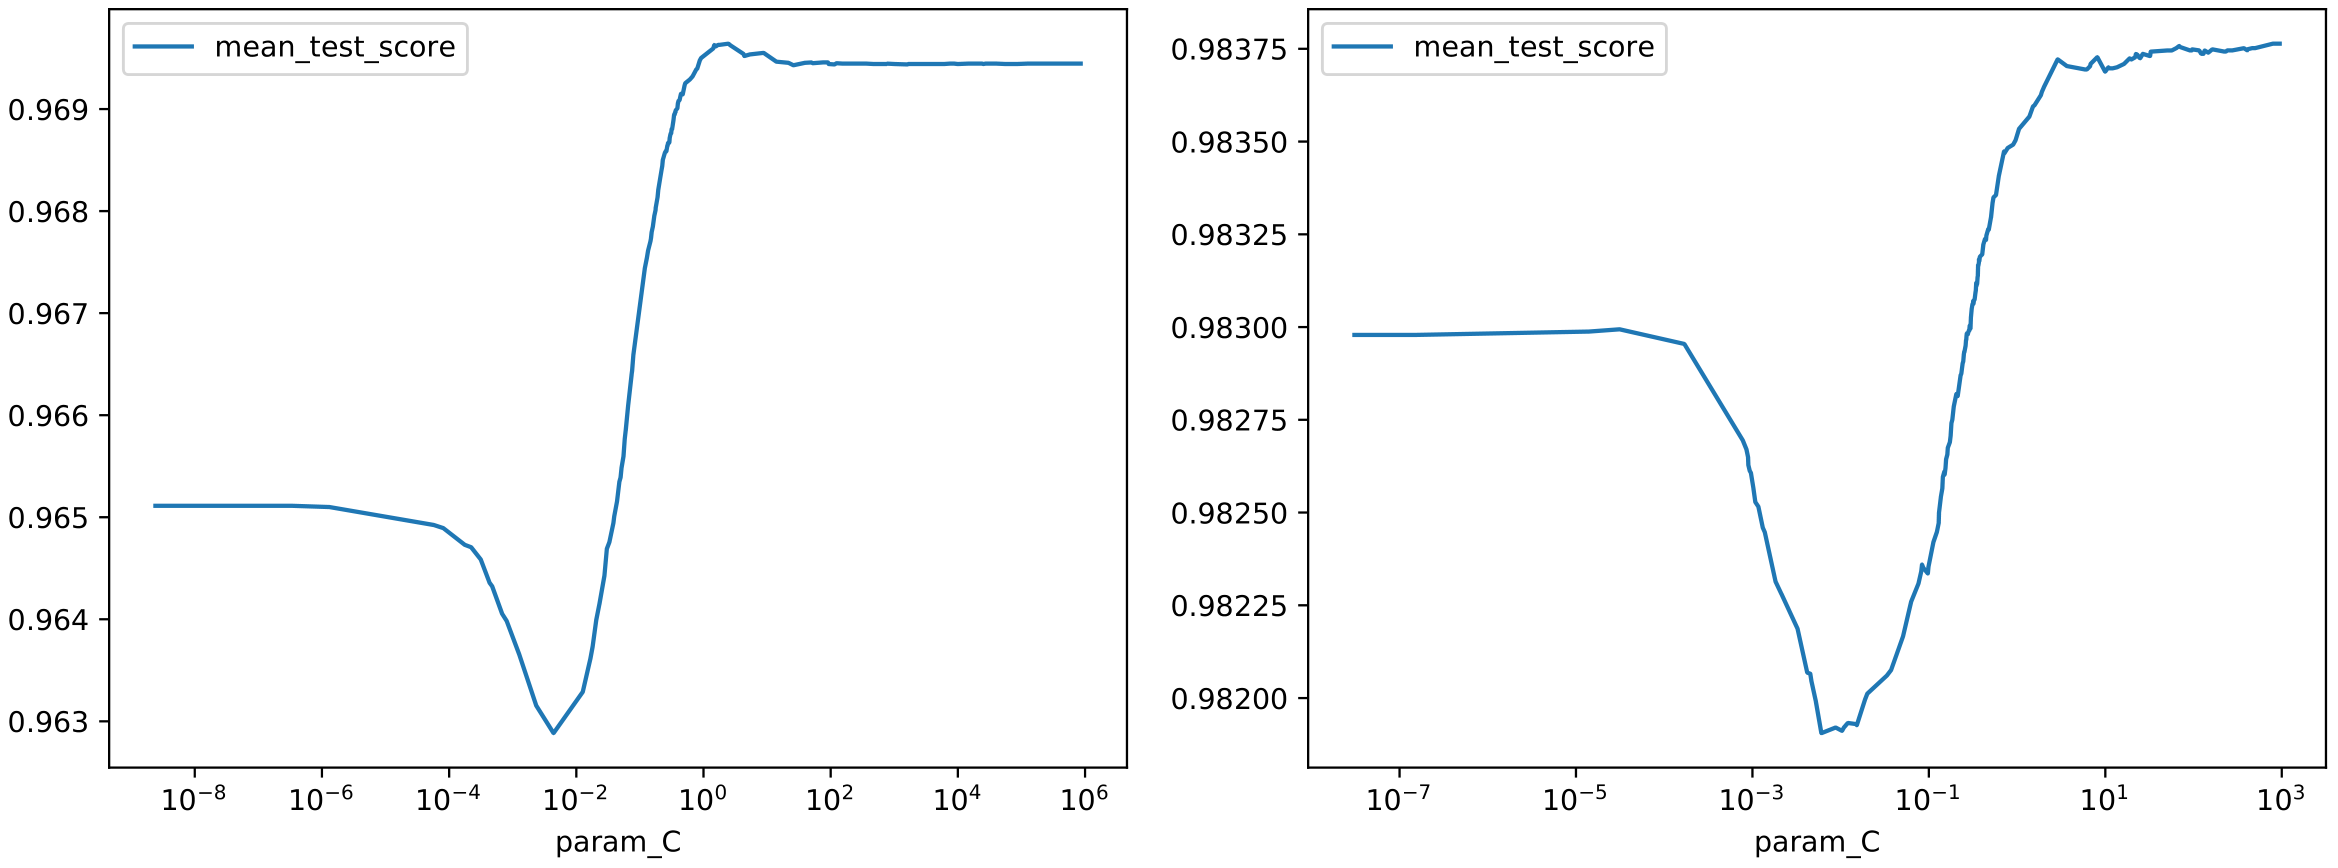
\includegraphics[width=15cm, height=6cm]{graphics/c_values.PNG}
		\caption{вредности регуларизационог параметра применом Бајесове претраге. (\textit{лево}) већи тренинг скуп (\textit{десно}) мањи тренинг скуп}
		\label{fig:c}
	\end{figure}

\section{Резултати}
	У табели \ref{table:results} се може видети да модел има одзив $0.72$ на позитивној класи и $F_1$ меру $0.81$, за случај поделе скупа података $80/10/10$. На тест скупу од $441$ инстанци, модел постиже укупну прецизност $94\%$.
	\begin{table}[h]
		\centering
		\begin{tabular}{SSSSS} \toprule
			{} & {прецизност} & {одзив} & {$F_1$} & {носач} \\ \midrule
			0  & 0.93 & 0.99 & 0.96 & 360 \\ 
			1  & 0.92  & 0.72 & 0.81 & 81 \\ \bottomrule
		\end{tabular}
		\caption{резултати на тест скупу}
		\label{table:results}
	\end{table}

\section{Закључак}
	На основу приказаних резултата, имплицитни приступ се показао као бољи. Исход је очекиван имајући у виду напреднији начин одређивања релевантности и коришћења те информације у оквиру самог модела. Чак и ако експлицитни приступ обезбеђује сличне карактеристике, моделу се ни једног тренутка не даје информација о важности атрибута већ се то мора закључити на основу сирових података.
	
	Постигнути су резултати који имају одличан одзив и $F_1$ меру над позитивном класом, што је и био циљ. За очекивати је да би успешност модела била већа када би скуп података био већи.

\section{Имплементација}
	Сав к\^{о}д се може наћи на страници GitHub \hyperref{http://www.github.com/4eyes4u/HRAnalytics}{category}{name}{репозиторијума}.

\end{document}